\problem{}
Jack wants to use carpets to cover the floor of the Student Activity Center. However, he can only find small carpets with certain special shapes.  He also needs to leave a given cell of the floor uncovered, which will be used for placing a bulletin board.
\begin{itemize}
    \item The floor of the Student Activity Center is a square shape where each side has length $n$, giving a total area of $n^{2}$ units.  You can assume $n = 2^{k}$ for some $k \geq 2$.
    \item There are four shapes of carpets, and each covers three unit cells of the floor. The shapes are shown below.
    \item The bulletin board will be put in one cell of the floor, and takes $1$ unit of area.
    \item All other cells without the bulletin board need to be covered by exactly one carpet. In another word, two carpets cannot overlap.
\end{itemize}
\begin{figure}[h]
     \centering
     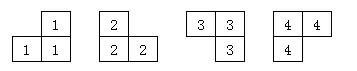
\includegraphics[width=0.6\textwidth]{figure/p5f1.png}
     \label{fig:carpet}
\end{figure}

As simple example, suppose the floor is a $2 \times 2$ square, and the bulletin board is placed in cell $(0,0)$.  Then we can use one carpet with shape 1 to cover the floor. \\

Given an algorithm for Jack to solve the problem with an $n \times n$ floor, where the bulletin board is placed in cell $(x,y)$, for $0 \leq x, y \leq n-1$.  Clearly describe your algorithm and why it is correct, and use pseudocode if necessary. \\

\emph{Hint}: Using divide-and-conquer, and consider the problem for a $4\times4$ floor first.

\solution{

}

\newpage